% !TEX root = 00_arbeit.tex

%---------------------------------------------------------------------------------
%% Anhang

%-------------------------------------------
%% Resettet den Abbildungszähler
%% Quelle:https://stackoverflow.com/questions/3391540/renumbering-figure-in-latex
\makeatletter 
\renewcommand{\thefigure}{A-\@arabic\c@figure}
\makeatother
\setcounter{figure}{0}

\section{Anhang}

\subsection{XOR bzw. exklusiv Oder}\label{sec:XOR}

\begin{figure}[!h]
\centering
\begin{circuitikz}
\draw (0,0)         node[european xor port] (xor)   {} 
      (xor.in 1)    node[left]                      {A}
      (xor.in 2)    node[left]                      {B}
      (xor.out)     node[right]                     {Y}
      ;
\end{circuitikz}
%\includegraphics{test}
\hspace{1cm}
\begin{tabular}{cc|c}
A & B & Y \\
\hline
0& 0 & 0 \\
0& 1 & 1 \\
1& 0 & 1 \\
1& 1 & 0 
\end{tabular}
\caption{Blockschaltbild des XOR-Gatters links und rechts die zugehörige Wahrheitstabelle.}
\label{fig_a:XOR}
\end{figure}

Das exklusive Oder bzw. XOR-Gatter ist ein Begriff aus dem Bereich der Logik. Mit der Gleichung:%
%
$$Y=\left ( \overline{A}  \land B \right)\lor \left ( A \land \overline{B} \right ).$$
Der Ausgang dieses Gatters ist dann~\glqq 1\grqq~wenn eine ungerade Anzahl an Eingängen auf~\glqq 1\grqq~liegt und die restlichen auf~\glqq 0\grqq. Das Blockschaltbild und die Wahrheitstabelle sind in \autoref{fig_a:XOR} dargestellt.

\todo{AND/OR funktion hinzufügen}

\subsection{Lernalgorithmen}
An dieser Stelle werden die Deltaregel und das Backpropagation-Verfahren hergeleitet.\,\footnote{Vgl. \citet[79 ff]{dkriesel07} und \citet[322 ff]{Rumelhart1986}.}


\subsubsection{Deltaregel}\label{sec:deltaregel}
%\todo{Perceptron-Lernalgorithmus}
    %http://www.theprojectspot.com/tutorial-post/introduction-to-artificial-neural-networks-part-2-learning/8

\todo{Grafik: SLP mit Linearer Aktivierungsfunktion und Abkürzungsübersicht}

Dargestellt ist ein Einschichtigesperceptron mit lierarer Aktikvierungsfunktion.
Zunächst wird die Verarbeitung von Informationen in dem in \farbig{Abbildung ??} dargestellten Netzwerk betrachtet. Die Information jedes Eingabeneurons $x_i$ wird mit einem Gewicht $w_{ij}$ versehen und an das Ausgabeneuron weitergeleitet. Die Propagierungsfunktion (die in diesem Fall die Summe darstellt) verarbeitet die Eingabe zu Netzeingabe $net_j$
\begin{equation}
net_j= \sum^{i=1}_n w_{ij} x_i
\end{equation}
und reicht diese an die Aktivierungsfunktion $f_{akt}$ weiter. Das Ergebniss der Aktivierungsfunktion ist dann die Ausgabe $o_j$ des Ausgabeneurons $j$
\begin{equation}
o_j= f_{akt}(net_j).
\end{equation}
Eine lineare Aktivierungsfunktion ergibt als Ausgabe eine Identität und somit ist
\begin{equation}
o_j= net_j= \sum_{i=1}^n w_{ij} x_i.
\label{gl:ausgang}
\end{equation}

Nun Soll das Netzwerk mit einer Menge an Trainingsbeispielen $P$ trainiert werden. Wobei die Menge $P$ sich aus einem Trainingsbeispiel $p$ und der zugehörigen Lösung $t$ also $(p,t)$ zusammensetzt.
Das Ziel des Trainings ist nun, dass die Ausgabe $o$ bei allen Trainingsbeispielen sich der zugehörigen Lösung $t$ möglichst angleicht bzw. die Differenz $\delta$ (auch als Fehler bezeichnet) 
\begin{equation}
\delta=t-o
\label{gl:delta}
\end{equation}

aus Lösung und Ausgabe möglichst klein  wird, also soll formal gelten
\begin{equation*}
\forall p:o \approx t \quad \text{bzw.} \quad \forall p:\delta \approx 0.
\end{equation*}

Bei einem Netzwerk mit zwei Eingabeneuronen und einem Ausgabeneuron (ergo zwei Gewichten) für ein Trainingsbeispiel eine Fehlerfläche $Err_p(W)$ (dargestellt in \autoref{fig:Fehlerlandschaft}), wobei $W$ die Menge aller Gewichte darstellt.

%\todo{Grafik: Fehlerfläche \citet[80]{dkriesel07}}
\begin{figure}[tb]
    \centering
        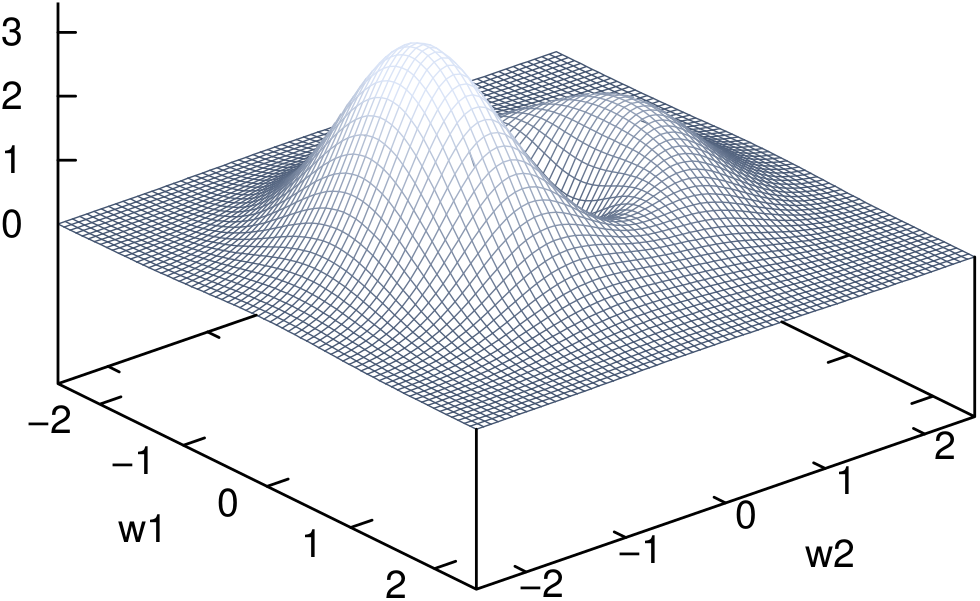
\includegraphics[width=0.5\textwidth]{Bilder/misc/Fehlerlandschaft.png}
    \caption{Beispiel einer Fehlerfläche eines Neuronalen Netzes mit zwei trainierbaren Gewichten. Bei weiteren Gewichten entsteht pro Gewicht eine zusätzliche Dimension in der Fehlerlandschaft. Was zu höherer Komplexität und zerklüfteter \glqq Oberfläche\grqq führt.\protect\footnotemark{}}
    \label{fig:Fehlerlandschaft}
\end{figure}
\addtocounter{footnote}{-1}     %  -1 mal die Gesamtanzahl an Fußnoten in der wrapfigure
\addtocounter{Hfootnote}{-1}    % -1 times total number of footnote(mark)s in the wrapfigure
\wrapfigfoot\footnotetext{\autoref{fig:Fehlerlandschaft} wurde aus \citet[80]{dkriesel07} übernommen.}

Durch anwendung des Gradientenabstigverfahrens\,\citef[63 f]{dkriesel07} kann nun vom Ausgangspunkt gesehen das nächste Minimum gefunden werden. Mit
\begin{equation}
\Delta w = - \alpha \nabla Err(W)
\end{equation}
erhält man nun die Information wie die Gewichte verändert werden können, um das Fehlerminimum zu finden.
Wobei $\alpha$ eine Proportionalitätskonstante darstellt, welche für die Schrittweite beim Gradientenabstieg verantwortlich ist.
Um zu erfahren wie jedes Gewicht verändert werden soll muss die Fehlerfunktion $Err(W)$ nach dem entsprechenden Gewicht $w_{ij}$ abgeleitet werden
\begin{equation}
\Delta w_{ij} = - \alpha \frac{\partial Err(W)}{\partial w_{ij}} .
\label{gl:gewaend}
\end{equation}

Die Fehlerfunktion $Err_p(W)$ für ein Trainingsbeispiel $p$ lässt sich auf unterschiedliche Weise bestimmen\,\footnote{\citet[60 f]{dkriesel07} gibt hierfür einige Beispiele an.}, an dieser Stelle wird der quadratische Abstand genutzt. Damit kann die Fehlerfunktion über alle Ausgabeneuronen berechnet werden mit:
\begin{equation}
Err_p(W)= \frac{1}{2} \sum^k_{j=1} (t_{pj}-o_{pj})^2 .
\end{equation}
Somit reduziert sich die Fehlerfunktion bei der Betrachtung eines Ausgabeneurons $j$ für ein Trainingsbeispiel $p$ zu
\begin{equation}
Err_p(W)= \frac{1}{2} (t_{pj}-o_{pj})^2 .
\label{gl:errp}
\end{equation}


Dabei entspricht bei dem Onlinelernen der Gesamtfehler $Err(W)$ dem Einzelfehler $Err_p(W)$
\begin{equation}
Err(W)=Err_p(W) 
\end{equation}
und bei dem Offlinelernen müssen die Einzelfehler aufsummiert werden
\begin{equation}
Err(W)= \sum^P_{p=1} Err_p(W). 
\end{equation}

Da in der \autoref{gl:errp} $t_{pj}$ konstant ist hängt $Err_p(W)$ nur von $o_{pj}$ ab. So kann die Ableitung $\frac{\partial Err_p(W)}{\partial w_{ij}}$ mit der Kettenregel zerlegt werden in
\begin{equation}
\frac{\partial Err_p(W)}{\partial w_{ij}}= \frac{\partial Err_p(W)}{\partial o_{pj}} \cdot \frac{\partial o_{pj}}{\partial w_{ij}}.
\label{gl:zerlket}
\end{equation}

Durch das Ableiten(\farbig{evtl. Differentitation}) der \autoref{gl:errp} nach $o_{pj}$ und einsetzen von \autoref{gl:delta} erhält man
\begin{equation}
\frac{\partial Err_p(W)}{\partial o_{pj}} = -(t_{pj}-o_{pj}) = - \delta_{pj} .
\label{gl:minusdelta}
\end{equation}

Unter Betrachtung der \autoref{gl:ausgang} kann der Ausdruck $ \frac{\partial o_{pj}}{\partial w_{ij}}$ nun auch geschrieben werden als 
\begin{equation}
\frac{\partial o_{pj}}{\partial w_{ij}} = \frac{\partial \sum\limits_{i=1}^n w_{ij} x_{pi}}{\partial w_{ij}} .
\label{gl:vor_xi}
\end{equation}
Wobei die abzuleitende Funktion zwar aus vielen Summanden zusammengesetzt ist aber nur der Summand $w_{ij} x_{pi}$ enthält die Variable $w_{ij}$ nach der abgeleitet wird. Es gilt also
\begin{equation}
\frac{\partial o_{pj}}{\partial w_{ij}} = x_{pi}.
\label{gl:xi}
\end{equation}
Durch das Einsetzen der \autoref{gl:xi} und \autoref{gl:minusdelta} in \autoref{gl:zerlket} erhält man:
\begin{equation}
\frac{\partial Err_p(W)}{\partial w_{ij}}= - \delta_{pj} \cdot x_{pi}.
\label{gl:ze}
\end{equation}
Somit kann mit der \autoref{gl:gewaend} die Deltaregel für das Onlinelernverfahren bestimmt werden:
\begin{equation}
\Delta w_{ij} = \alpha \cdot \delta_{pj} \cdot x_{pi} .
\label{gl:fertig_delta}
\end{equation}
Für das Offlinelernverfahren muss noch die Summe über alle Trainingsbeispiele gebildet werden
\begin{equation}
\Delta w_{ij} = \alpha \cdot \sum^P_{p=1} \delta_{pj} \cdot x_{pi} .
\end{equation}



\subsection{Ergebnisse von \citet{Aggarwal2009} und \citet{Panapakidis2016}}\label{sec:andere_ergebnisse}

\todo{Liste der Märkte aus \citet{Cerjan2013}}

\todo{Tabellen einfügen und Hinweiß dass SVM keine ANN sind}

\subsection{Performancemaße}\label{sec:perfmas}
In diesem Abschnitt werden die Maße zur Evaluierung der Vorhersagegenauigkeit (weiterhin als Performancemaße bezeichnet) aufgeführt die in der Literaturrecherche zur Strompreismodellierung in \autoref{sec:strompreis} und weiterer Literatur\,\citef[5]{Guertler2017} genannt wurden. Hierbei $y_i$ und $\hat{y}_i$ die tatsächlichen und vorhergesagten Preise zum Zeitpunkt $i$ darstellen und $T$ die Gesamtanzahl der Zeitpunkte angibt. Außerdem gibt $\mean{y}$ den Mittelwert der tatsächlichen Preise und $\mean{y}_{train}$ den Preismittelwert der Trainingsdaten an.

Der Absolute Percentage Error (APE) liefert Informationen über die Fehlerverteilung in der Nähe der Null.\,\citef[14\label{foot:Domanski2017}]{Domanski2017}\farbig{reicht noch nicht}

% APE
\begin{equation}
APE= \sum\limits_{i \in T} \frac{\abs{y_i-\hat{y}_i}}{y_i}.
\label{gl:APE}
\end{equation}


Der Mean Absolute Percentage Error (MAPE) gibt einen prozentualen Mittelwert über den Fehlerbetrag an. Da das Ursprungsmaß (in dieser Arbeit als $MAPE_1$ bezeichnet) bei sehr kleinen Preisen einen hohen Werte liefert und bei einem Preis von Null sogar gegen Unendlich gehen wurden Mehrere Verbesserungen vorgeschlagen. Diese äußern sich durch einen Mittelwert über alle gemessenen Preise bei $MAPE_2$ oder durch einen Mittelwert aus der Betragssumme der des tatsächlichen und vorhergesagten Preises bei $sMAPE$ im Nenner. Hierbei steht ein Wert von 0\,\% für eine exakte und Werte um die 10\,\% für eine akkurate Vorhersage.\,\footnote{Vgl. \citet[17]{Bobinaite2016}, \citet[2105]{Amjady2009} und \citet[894]{Lago2018}.}   
% MAPE
\begin{equation}
MAPE_1= \frac{100}{T} \sum\limits_{i \in T} \frac{\abs{y_i-\hat{y}_i}}{y_i},
\label{gl:MAPE_1}
\end{equation}

% MAPE
\begin{equation}
MAPE_2= \frac{100}{T} \sum\limits_{i \in T} \frac{\abs{y_i-\hat{y}_i}}{\mean{y}},
\label{gl:MAPE_2}
\end{equation}

% sMAPE
\begin{equation}
sMAPE= \frac{100}{T} \sum\limits_{i \in T} \frac{\abs{y_i-\hat{y}_i}}{(\abs{y_i} + \abs{\hat{y}_i}) / 2}.
\label{gl:sMAPE}
\end{equation}

Der Mean Squared Error (MSE) gibt den quadratischen Mittelwert der der Fehler an und gibt an wie weit die vorhergesagten Daten von den tatsächlichen Werten liegen. Ein kleine Wert deutet auf eine gute vorhersage hin.\,\footnoteref{foot:Domanski2017}
% MSE
\begin{equation}
MSE= \frac{1}{T} \sum\limits_{i \in T} (y_i-\hat{y}_i)^2.
\label{gl:MSE}
\end{equation}


Der Root Mean Squared Error (RMSE) ist die Quadratwurzel des MSE und ist hierdurch sehr ähnlich. Der RMSE weist kleinere Werte auf, der Aussagegehalt ist aber ähnlich zu MSE.
% RMSE
\begin{equation}
RMSE= \sqrt{ \frac{1}{T} \sum\limits_{i \in T} (y_i-\hat{y}_i)^2}.
\label{gl:RMSE}
\end{equation}

Der Mean Absolut Error (MAE) ist ebenfalls sehr ähnlich zum MSE und damit auch dem RMSE. Weist aber im Vergleich zum RMSE nochmals kleinere Werte auf.
% MAE
\begin{equation}
MAE= \frac{1}{T} \sum\limits_{i \in T} \abs{y_i-\hat{y}_i}.
\label{gl:MAE}
\end{equation}


Der Normalized Mean Square Error (NMSE) ist ein Schätzwert über alle Abweichungen zwischen vorhergesagten und gemessenen Werten. Zeigt ein Modell einen sehr geringen NMSE so weist es eine gute örtliche und zeitliche Performance auf. Andererseits bedeuten hohe $NMSE$-Werte nicht, dass das betrachtete Modell komplett falsch ist.
% NMSE
\begin{gather}
\begin{aligned}
NMSE &= \frac{1}{\Delta^2 T} \sum\limits_{i \in T} (y_i-\hat{y}_i)^2,\\ 
\Delta^2 &= \frac{1}{T-1} \sum\limits_{i \in T} (y_i-\mean{y})^2.\\
\end{aligned}
\label{gl:NMSE}
\end{gather}


Die Error Variance (EV) gibt einen Wert über die nicht erklärten Informationen nach dem Fitten des Modells. Je kleiner der Wert ist desto präziser ist die Vorhersage.\,\citef{Peter2016}
% EV
\begin{equation}
EV= \sigma^2 = \frac{1}{T} \sum\limits_{i \in T} \left ( \frac{\abs{y_i-\hat{y}_i}}{\mean{y}} - MAPE_2  \right ) ^2.
\label{gl:EV}
\end{equation}

Pearson Korrelationskoeffizient bewertet die Linearität zwischen der Kovarianz zweier Variablen und dem Produkt der Standardabweichung dieser Variablen. Der Wertebereich dieses Maßes ist [-1,1] und er gibt Auskunft, wie Ähnlich der zeitliche Verlauf zwischen dem tatsächlichen Preis und der Vorhersage ist. Ein Wert von Eins deutet auf eine perfekte vorhersage hin.\,\citef{Davo2016} 
% cor
\begin{equation}
cor = \frac{cov(y_i,\hat{y}_i)}{\sqrt{sd(y_i)sd(\hat{y}_i)}} .
\label{gl:cor}
\end{equation}


Theils Koeffizienten der Ungleichheit U1 und U2 unterscheiden sich in der Anwesenheit bzw. Abwesenheit eines $\hat{y}_i$ im Nenner. Hierbei steht der Wert von Null in beiden fällen für Gleichheit und somit für eine ideale Vorhersage. Bei einem Wert von Eins spricht man von einer maximalen Ungleichheit. Dies kann bei U1 der Fall sein wenn eine negative Proportionalität besteht oder einer der Terme im Nenner Null ist. Bei dem U2 kann dies der Fall sein, wenn die Vorhersagemethode eine \textit{Na\"{i}ve-No-Change-Extrapolation}\,\citef[6]{Lattyak2011} ist oder wenn U2 zu der gleichen Standardabweichung des Prognosefehlers führt wie die Vorhersagemethode.\,\citef[444 f]{Bliemel1973}
% U1
\begin{equation}
U1 = \frac{\sqrt{\frac{1}{T} \sum_{i \in T} (y_i-\hat{y}_i)^2}}{ \sqrt{\frac{1}{T} \sum_{i \in T} y_i^2} + \sqrt{\frac{1}{T} \sum_{i \in T} \hat{y}_i^2}},
\label{gl:U1}
\end{equation}

% U2
\begin{equation}
U2 = \frac{\sqrt{\sum_{i \in T} (y_i-\hat{y}_i)^2}}{ \sqrt{ \sum_{i \in T} y_i^2} }.
\label{gl:U2}
\end{equation}


Das out-of-sample (R²) Bestimmtheitsmaß ist dem Relative Absolute Error (RAE) sehr ähnlich. Wenn das RAE kleiner 100 und das R² größer Null ist, so ist die Vorhersagegenauigkeit höher als der historische Mittelwert der Trainingsdaten.
% R²
\begin{equation}
R^2 = 1 -  \frac{\frac{1}{T} \sum_{i \in T} \abs{y_i-\hat{y}_i}^2}{ \frac{1}{T} \sum_{i \in T} \abs{y_i-\mean{y}_{train}}^2 } ,
\label{gl:R2}
\end{equation}


% RAE
\begin{equation}
RAE = \frac{\frac{1}{T} \sum_{i \in T} \abs{y_i-\hat{y}_i}}{ \frac{1}{T} \sum_{i \in T} \abs{y_i-\mean{y}_{train}} } \cdot 100 .
\label{gl:RAE}
\end{equation}


Der Absolute Error (ABS) und der Relative Error (REL) wertet den systematischen Fehler aus. Der Idealwert ist hierbei Null, wobei dies mit einer exakten Vorhersage gleichzusetzen ist. Positive Werte weisen dabei auf eine Überschätzung und negative auf eine Unterschätzung der Vorhersage hin.\,\citef[5 f]{Guertler2017}

% ABS
\begin{equation}
ABS= \frac{1}{T} \sum\limits_{i \in T} (\hat{y}_i-y_i),
\label{gl:ABS}
\end{equation}


% REL
\begin{equation}
REL= \frac{\sum_{i \in T} (\hat{y}_i-y_i)}{\sum_{i \in T} y_i} .
\label{gl:REL}
\end{equation}



\begin{figure}[!htb]
    \centering
        
\pgfplotsset{every axis/.append style={
                label style={font=\footnotesize},
                tick label style={font=\footnotesize},
                x label style={yshift=.5em},
            }}
%%--------------------MAPE-MAE-RAE-------------------------%%
 \begin{tikzpicture}
 
    \def\datafile{Daten/BP/logist/m/BP_logis_m-epochen.dat}
 
    \pgfplotsset{
        %scale only axis,
        minor x tick num=1,
        xmin=0, xmax=51,
        width=15cm,
        height=8cm,
        ylabel style={rotate=180},
        xticklabel style={
            /pgf/number format/precision=3,
            /pgf/number format/fixed,
            x label style={yshift=.5em},
        },
    }
 
    \begin{axis}[
    axis y line*=left,
    xlabel=Epochen,
    ylabel=MAPE,
    y label style={yshift=.5em},
    %xlabel near ticks,
    minor y tick num=1,
    ]
    \addplot[
    mark=none,
    draw=green,
    ] 
    table[
    /pgf/number format/read comma as period,
    x=epochen, 
    y=MAPE_mean, 
    col sep=tab,
    ] {\datafile};
    \label{MAPE-}


       %\addplot[pattern=crosshatch,pattern color=blue!30!white,draw=blue!30!white]{x^2} \closedcycle;
       %\addplot[red,line legend] coordinates {(0,0) (1,1)};
       %\legend{RMSE,U2}
    \end{axis}

    \begin{axis}[
    axis x line=none,
    axis y line*=left,
    ylabel=MAE,
    y label style={yshift=.5em},
    minor y tick num=1,
    ] 
    %\addlegendimage{/pgfplots/refstyle=MAPE}\addlegendentry{MAPE}
    \pgfplotsset{
        every outer y axis line/.style={xshift=-1.2cm}, 
        every tick/.style={xshift=-1.2cm}, 
        every y tick label/.style={xshift=-1.2cm} 
    }
    
    \addplot[
    mark=none,
    draw=purple,
    ] 
    table[
    /pgf/number format/read comma as period,
    x=epochen, 
    y=MAE_mean,
    col sep=tab,
    ] {\datafile};
    \label{MAE-}
    \end{axis}
    
    \begin{axis}[
    axis x line=none,
    axis y line*=right,
    ylabel=RAE,
    y label style={yshift=-.5em},
    minor y tick num=1,
    ] 
    \addlegendimage{/pgfplots/refstyle=MAPE-}\addlegendentry{MAPE}
    \addlegendimage{/pgfplots/refstyle=MAE-}\addlegendentry{MAE}

    \addplot[
    mark=none,
    draw=cyan,
    ] 
    table[
    /pgf/number format/read comma as period,
    x=epochen, 
    y=RAE_mean, 
    col sep=tab,
    ] {\datafile};
    \addlegendentry{RAE}
    \end{axis}

   \end{tikzpicture}
    \caption{Gegenüberstellung des $MAPE$, des $MAE$ und des $RAE$ wobei auffällt, dass die Maße sich in einem Faktor unterscheiden.}
    \label{fig:geg_mape_mae_rae}
\end{figure}

\begin{figure}[!htb]
    \centering
        \pgfplotsset{every axis/.append style={
                label style={font=\footnotesize},
                tick label style={font=\footnotesize},
                x label style={yshift=.5em},
            }}

%%--------------------RMSE-U2----------------------------%%
 \begin{tikzpicture}
 
    \def\datafile{Daten/BP/logist/m/BP_logis_m-epochen.dat}
 
    \pgfplotsset{
        %scale only axis,
        minor x tick num=1,
        xmin=0, xmax=51,
        width=15cm, %\textwidth,
        height=8cm,
        ylabel style={rotate=180},
        xticklabel style={
            /pgf/number format/precision=3,
            /pgf/number format/fixed,
        },
    }
 
    \begin{axis}[
    axis y line*=left,
    xlabel=Epochen,
    ylabel=RMSE,
    y label style={yshift=.5em},
    %xlabel near ticks,
    minor y tick num=1,
    ]
    \addplot[
    mark=none,
    draw=black,
    ] 
    table[
    /pgf/number format/read comma as period,
    x=epochen, 
    y=RMSE_mean, 
    col sep=tab,
    ] {\datafile};
    \label{RMSE-}

    \end{axis}

    \begin{axis}[
    axis x line=none,
    axis y line*=right,
    ylabel=U2,
    y label style={yshift=-.5em},
    minor y tick num=1,
    ] 
    \addlegendimage{/pgfplots/refstyle=RMSE-}\addlegendentry{RMSE}
    %\pgfplotsset{
    %    every outer y axis line/.style={xshift=-1.2cm}, 
    %    every tick/.style={xshift=-1.2cm}, 
    %    every y tick label/.style={xshift=-1.2cm} 
    %}
    
    \addplot[
    mark=none,
    draw=red,
    ] 
    table[
    /pgf/number format/read comma as period,
    x=epochen, 
    y=U2_mean, 
    col sep=tab,
    ] {\datafile};
    \addlegendentry{U2}
    \end{axis}

   \end{tikzpicture}
    \caption{Die gleiche Beobachtung wie in \autoref{fig:geg_mape_mae_rae} kann auch bei der Gegenüberstellung des $RMSE$ und des $U2$ gemacht werden.}
    \label{fig:geg_rmse_u2}
\end{figure}

\begin{landscape}
\begin{figure}[!htb]
    \centering
        \pgfplotsset{every axis/.append style={
                label style={font=\footnotesize},
                tick label style={font=\footnotesize},
                x label style={yshift=.5em},
            }}
%%--------------------alle-------------------------%%
 \begin{tikzpicture}
 
    \def\datafile{Daten/BP/logist/m/BP_logis_m-epochen.dat}

    \def\xshiftlab{1.1cm}
 
    \pgfplotsset{}
 
    \pgfplotsset{
        %scale only axis,
        minor x tick num=1,
        xmin=0, xmax=51,
        width=15cm, %\textwidth,
        height=13cm,
        ylabel style={rotate=180},
        xticklabel style={
            /pgf/number format/precision=3,
            /pgf/number format/fixed},
        every axis legend/.append style={
        at={(0.5,1.03)},
        anchor=south},
    }
 %%----------------------RMSE-----------------------------%%
    \begin{axis}[
    axis y line*=left,
    xlabel=Epochen,
    ylabel=RMSE,
    y label style={yshift=.5em},
    xlabel near ticks,
    minor y tick num=1,
    ]
    \addplot[
    mark=none,
    draw=black,
    ] 
    table[
    /pgf/number format/read comma as period,
    x=epochen, 
    y=RMSE_mean, 
    col sep=tab,
    ] {\datafile};
    \label{RMSE}
    \end{axis}

%%------------------------U2------------------------------%%
    \begin{axis}[
    axis x line=none,
    axis y line*=left,
    ylabel=U2,
    y label style={yshift=.75em},
    minor y tick num=1,
    ] 
    \pgfplotsset{
        every outer y axis line/.style={xshift=-\xshiftlab*1.2}, 
        every tick/.style={xshift=-\xshiftlab*1.2}, 
        every y tick label/.style={xshift=-\xshiftlab*1.2} 
    }
    
    \addplot[
    mark=none,
    draw=red,
    ] 
    table[
    /pgf/number format/read comma as period,
    x=epochen, 
    y=U2_mean, 
    col sep=tab,
    ] {\datafile};
    \label{U2}
    \end{axis}

%%------------------------REL------------------------------%%
    \begin{axis}[
    axis x line=none,
    axis y line*=left,
    ylabel=REL,
    y label style={yshift=.6em},
    minor y tick num=1,
    ] 
    \pgfplotsset{
        every outer y axis line/.style={xshift=-\xshiftlab*2.3}, 
        every tick/.style={xshift=-\xshiftlab*2.3}, 
        every y tick label/.style={xshift=-\xshiftlab*2.3} 
    }
    
    \addplot[
    mark=none,
    draw=orange,
    ] 
    table[
    /pgf/number format/read comma as period,
    x=epochen, 
    y=REL_mean, 
    col sep=tab,
    ] {\datafile};
    \label{REL}
    \end{axis}

%%------------------------ABS------------------------------%%
    \begin{axis}[
    axis x line=none,
    axis y line*=left,
    ylabel=ABS,
    y label style={yshift=.6em},
    minor y tick num=1,
    ] 
    \pgfplotsset{
        every outer y axis line/.style={xshift=-\xshiftlab*3.45}, 
        every tick/.style={xshift=-\xshiftlab*3.45}, 
        every y tick label/.style={xshift=-\xshiftlab*3.45} 
    }
    
    \addplot[
    mark=none,
    draw=lime,
    ] 
    table[
    /pgf/number format/read comma as period,
    x=epochen, 
    y=ABS_mean, 
    col sep=tab,
    ] {\datafile};
    \label{ABS}
    \end{axis}

%%------------------------EV------------------------------%%
    \begin{axis}[
    axis x line=none,
    axis y line*=left,
    ylabel=EV,
    y label style={yshift=.5em},
    minor y tick num=1,
    ] 
    \pgfplotsset{
        every outer y axis line/.style={xshift=-\xshiftlab*4.45}, 
        every tick/.style={xshift=-\xshiftlab*4.45}, 
        every y tick label/.style={xshift=-\xshiftlab*4.45} 
    }
    
    \addplot[
    mark=none,
    draw=brown,
    ] 
    table[
    /pgf/number format/read comma as period,
    x=epochen, 
    y=EV_mean, 
    col sep=tab,
    ] {\datafile};
    \label{EV}
    \end{axis}





%%----------------------sMAPE-----------------------------%%
    \begin{axis}[
    axis x line=none,
    axis y line*=right,
    %xlabel=Epochen,
    ylabel=sMAPE,
    y label style={yshift=-.5em},
    minor y tick num=1,
    ]
    \addplot[
    mark=none,
    draw=magenta,
    ] 
    table[
    /pgf/number format/read comma as period,
    x=epochen, 
    y=sMAPE_mean, 
    col sep=tab,
    ] {\datafile};
    \label{sMAPE}
    \end{axis}

%%----------------------MAPE-----------------------------%%
    \begin{axis}[
    axis x line=none,
    axis y line*=right,
    %xlabel=Epochen,
    ylabel=MAPE,
    y label style={yshift=-.5em},
    minor y tick num=1,
    ]
    
    \pgfplotsset{
        every outer y axis line/.style={xshift=\xshiftlab}, 
        every tick/.style={xshift=\xshiftlab}, 
        every y tick label/.style={xshift=\xshiftlab} 
    }
    
    \addplot[
    mark=none,
    draw=green,
    ] 
    table[
    /pgf/number format/read comma as period,
    x=epochen, 
    y=MAPE_mean, 
    col sep=tab,
    ] {\datafile};
    \label{MAPE}
    \end{axis}

%%----------------------MAE-----------------------------%%
    \begin{axis}[
    axis x line=none,
    axis y line*=right,
    ylabel=MAE,
    y label style={yshift=-.85em},
    minor y tick num=1,
    ] 
    %\addlegendimage{/pgfplots/refstyle=MAPE}\addlegendentry{MAPE}
    \pgfplotsset{
        every outer y axis line/.style={xshift=\xshiftlab*2}, 
        every tick/.style={xshift=\xshiftlab*2}, 
        every y tick label/.style={xshift=\xshiftlab*2} 
    }
    
    \addplot[
    mark=none,
    draw=purple,
    ] 
    table[
    /pgf/number format/read comma as period,
    x=epochen, 
    y=MAE_mean,
    col sep=tab,
    ] {\datafile};
    \label{MAE}
    \end{axis}

%%----------------------RAE-----------------------------%%
    \begin{axis}[
    axis x line=none,
    axis y line*=right,
    ylabel=RAE,
    y label style={yshift=-.5em},
    minor y tick num=1,
    ]

    \pgfplotsset{
        every outer y axis line/.style={xshift=\xshiftlab*3}, 
        every tick/.style={xshift=\xshiftlab*3}, 
        every y tick label/.style={xshift=\xshiftlab*3} 
    }

    \addplot[
    mark=none,
    draw=cyan,
    ] 
    table[
    /pgf/number format/read comma as period,
    x=epochen, 
    y=RAE_mean, 
    col sep=tab,
    ] {\datafile};
    \label{RAE}
    \end{axis}

%%----------------------R²-----------------------------%%
    \begin{axis}[
    axis x line=none,
    axis y line*=right,
    ylabel=R$^2$,
    y dir=reverse,
    y label style={yshift=-.5em},
    minor y tick num=1,
    legend columns=10,
    ]
    
    \addlegendimage{/pgfplots/refstyle=RMSE}\addlegendentry{RMSE}
    \addlegendimage{/pgfplots/refstyle=U2}\addlegendentry{U2}
    \addlegendimage{/pgfplots/refstyle=REL}\addlegendentry{REL}
    \addlegendimage{/pgfplots/refstyle=ABS}\addlegendentry{ABS}
    \addlegendimage{/pgfplots/refstyle=EV}\addlegendentry{EV}
    \addlegendimage{/pgfplots/refstyle=sMAPE}\addlegendentry{sMAPE}
    \addlegendimage{/pgfplots/refstyle=MAPE}\addlegendentry{MAPE}
    \addlegendimage{/pgfplots/refstyle=MAE}\addlegendentry{MAE}
    \addlegendimage{/pgfplots/refstyle=RAE}\addlegendentry{RAE}

    \pgfplotsset{
        every outer y axis line/.style={xshift=\xshiftlab*4}, 
        every tick/.style={xshift=\xshiftlab*4}, 
        every y tick label/.style={xshift=\xshiftlab*4} 
    }

    \addplot[
    mark=none,
    draw=blue,
    ] 
    table[
    /pgf/number format/read comma as period,
    x=epochen, 
    y=R2_mean, 
    col sep=tab,
    ] {\datafile};
    \addlegendentry{R2}
    \end{axis}

   \end{tikzpicture}
    \caption{Dargestellt ist die Messung der optimalen Epochenanzahl eines MLPs mit Bias-Neuron welches mit dem BP-Verfahren trainiert wird und eine logistische Aktivierungsfunktion besitzt. Dieser Graph dient der Gegenüberstellung aller in dieser Arbeit betrachteten Performancemaße.}
    \label{fig:geg_alle}
\end{figure}
\end{landscape}

%-----------------------------------------------------------------------------------
\todo{Fehlermaße aufführen und bedeutung erkären}